\thispagestyle{diendandayvahoctoannone}
\pagestyle{diendandayvahoctoan}
\everymath{\color{diendantoanhoc}}
\graphicspath{{../diendantoanhoc/pic/}}
\blfootnote{$^{1}$\color[named]{diendantoanhoc}Tòa soạn Hà Nội, Báo Thanh Niên.}
\begingroup
\AddToShipoutPicture*{\put(0,616){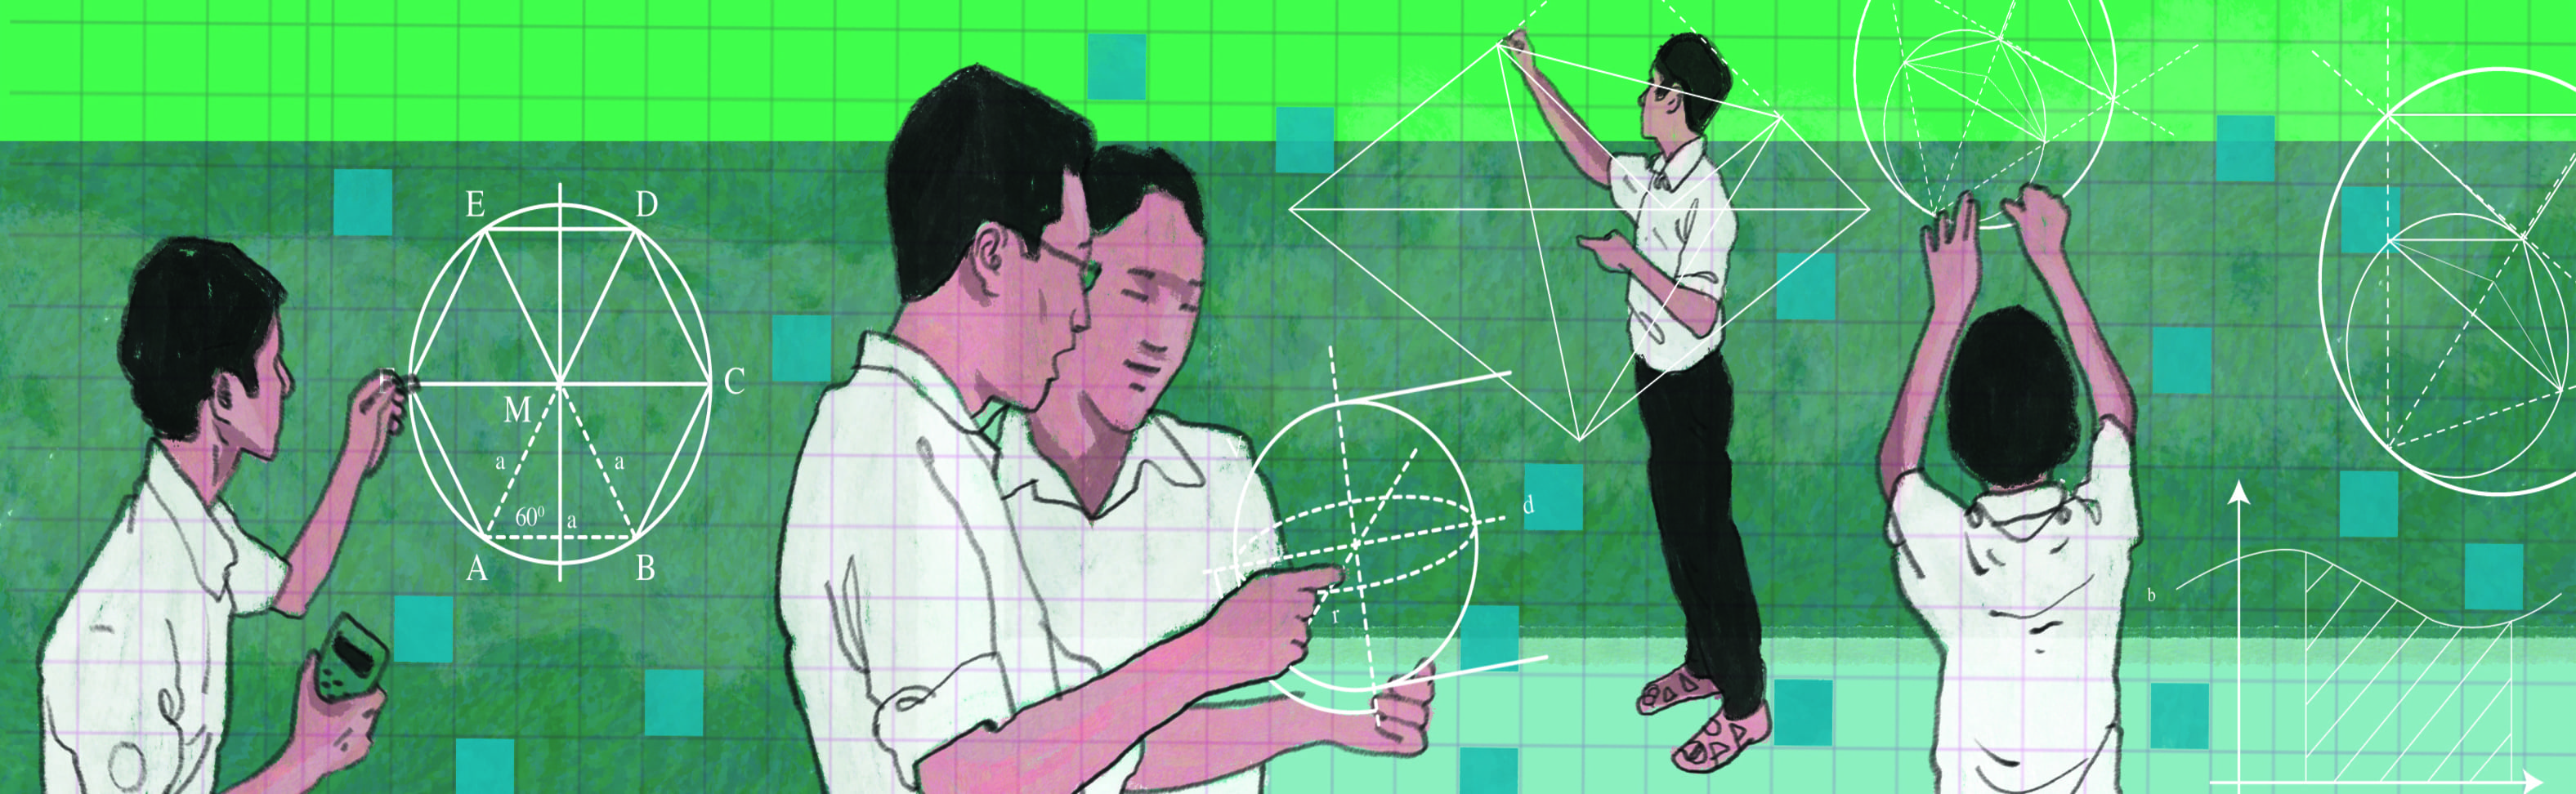
\includegraphics[width=19.3cm]{../bannerdiendan}}}
\AddToShipoutPicture*{\put(114,525){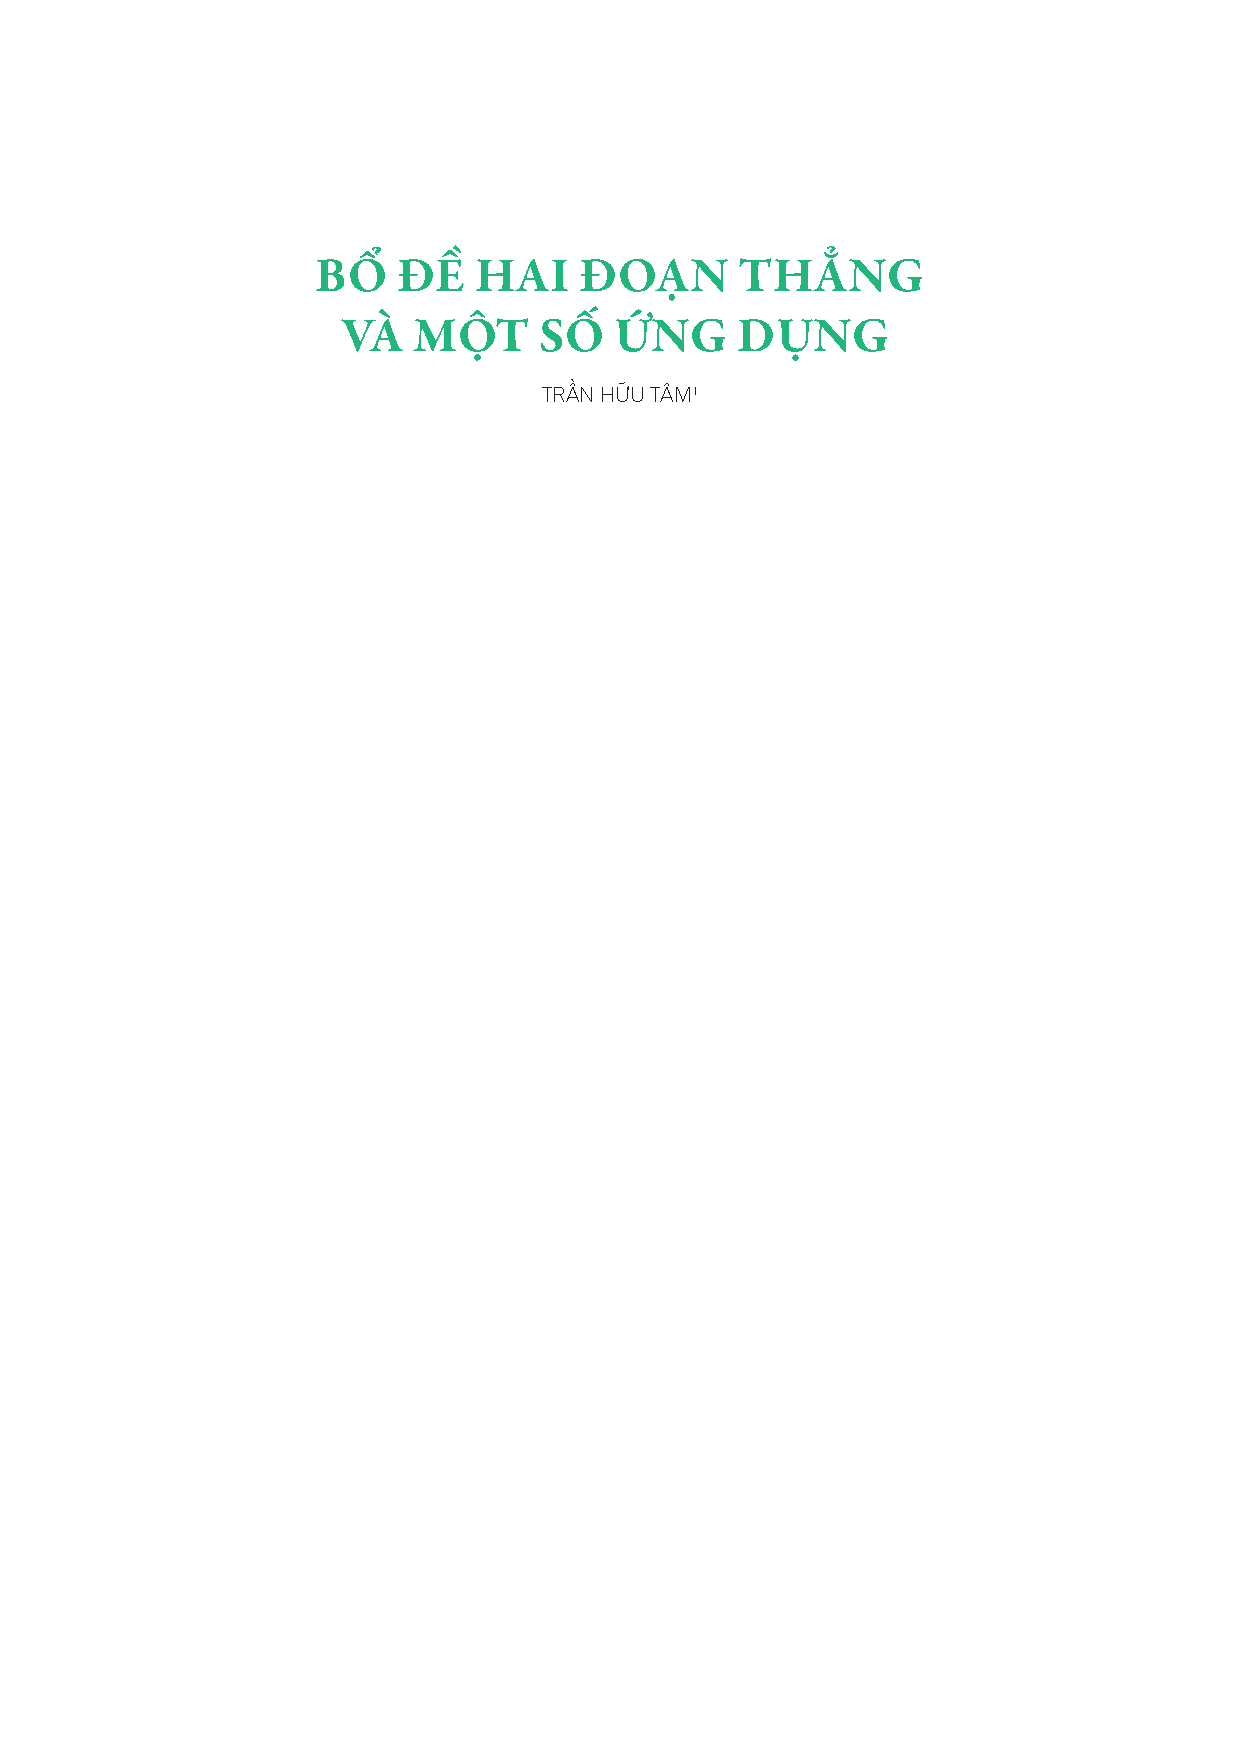
\includegraphics[scale=1]{../tieude.pdf}}}
\centering
\endgroup
\vspace*{188pt}

\textit{Với những ai quan tâm kỳ thi Bài giảng và bài viết về Toán học mang tên Hoàng Tụy, không chỉ là xem các thí sinh thuyết trình bài giảng, mà hơn thế, được nghe các thầy giám khảo chia sẻ quan điểm về dạy toán.}

\begin{multicols}{2}
	Theo nhận định của nhiều người theo dõi, điều lôi cuốn người xem nhất ở vòng chung khảo kỳ thi Bài giảng và bài viết về Toán học, mang tên Hoàng Tụy, là phần nhận xét của các thành viên hội đồng giám khảo. Nội dung các nhận xét này không chỉ đơn giản chỉ là những lời khen chê. Quan trọng hơn, đó là những chia sẻ về quan điểm dạy toán từ những giáo sư toán có sự am hiểu sâu sắc về toán phổ thông, thậm chí nhiều người trong đó đóng vai trò chủ chốt trong việc việc tham gia biên soạn chương trình phổ thông $2018$ như GS Đỗ Đức Thái, GS Phùng Hồ Hải. 
	\vskip 0.1cm
	\textbf{\color{diendantoanhoc}Dạy toán ứng dụng không dễ}
	\vskip 0.1cm
	Bài thuyết trình \textit{Lý thuyết đồ thị và một số cấu trúc đáng chú ý} của tác giả Hà Trung (Trường THPT chuyên Lê Hồng Phong, Nam Định) nhận được sự quan tâm đặc biệt của hội đồng giám khảo. Đây là chuyên đề (không bắt buộc) sẽ được dạy cho học sinh lớp $11$ của chương trình phổ thông $2018$ (bắt đầu được triển khai từ năm học $2023-2024$). Nhưng theo tác giả Hà Trung, lý do anh chọn chuyên đề này bởi nó có nhiều kiến thức thú vị, có nhiều ứng dụng trong cuộc sống (ví dụ bản đồ mạng lưới bay của hàng không, mạng tương tác gene). 
	\vskip 0.1cm
	Theo GS Phùng Hồ Hải thì việc tác giả ``gói" ba nội dung (sơ lược về lý thuyết đồ thị; đồ thị lưỡng phân; đồ thị cây, rừng) trong một chuyên đề là hơi ôm đồm. Hơn nữa, đối tượng mà người dạy là hướng đến học sinh giỏi toán, thì không cần thiết phải mất quá nhiều thời gian vòng vo về những ứng dụng mà nên đi thẳng sâu vào bản chất nội dung. 
	\vskip 0.1cm
	GS Ngô Việt Trung cho rằng, tác giả cần lựa chọn bài toán phù hợp với kiến thức đồ thị để giảng dạy. Không nên nhắc tới những vấn đề chỉ mang tính minh họa. Bài toán về chủ đề đồ thị thì mình phải áp dụng kiến thức đồ thị để giải quyết vấn đề. Chẳng hạn như nói về mạng thì kiến thức đồ thị đóng vai trò quan trọng. Ví dụ ChatGPT chắc chắn là phải dùng đồ thị để xác định những gì gắn với nhau. 
	\vskip 0.1cm
	Còn theo GS Đỗ Đức Thái, điều khiến cho đồ thị quan trọng hơn đối với toán học và đối với cuộc sống bây giờ là những thuật toán để từ đó giúp chúng ta tìm được câu trả lời. Chẳng hạn, người ta có thể mô tả  ở chu trình Ơ le thì có cái này, hoặc ở đồ thị lưỡng phân thì sẽ có cái thứ như thế này... Trong khi cái quan trọng phải là có thuật toán để tìm những cái đấy thế nào. Và thuật toán đó phải mô phỏng được, phải lập trình được để thành ra những cái chạy được trên máy tính. ``Có lẽ đến một lúc nào đó chúng ta nên dạy học sinh những cái như thế. Còn cứ gieo vào đầu học sinh, nhất là học sinh giỏi toán, rằng dùng cái này suy ra những cái trừu tượng này..., thì mãi cũng sẽ chẳng đi đến đâu. Cho nên tôi nghĩ nên chọn những bài toán, vẫn là toán hoàn toàn, vẫn khó như thường, nhưng cho phép người ta lập trình được, gắn vào một thuật toán nào đó coding được nó", GS Thái gợi ý. 
	\vskip 0.1cm
	\textbf{\color{diendantoanhoc}Dạy cho tử tế toán!}
	\vskip 0.1cm
	Với phần trình bày của tác giả Nguyễn Thế Minh (Trường Trung học Vinschool Imperia, Hải Phòng), chủ đề \textit{Tích hợp tư duy công dân số trong bài giảng môn Toán}, GS Đỗ Đức Thái cho rằng, bài giảng phù hợp với xu hướng tích hợp mà Chương trình phổ thông $2018$ muốn thúc đẩy. Thông qua kiến thức về toán, người dạy muốn mang đến cho người học những gợi mở ứng dụng trong lĩnh vực tin học, đó là ưu điểm của bài giảng. 
	\begin{figure}[H]
		\vspace*{-5pt}
		\centering
		\captionsetup{labelformat= empty, justification=centering}
		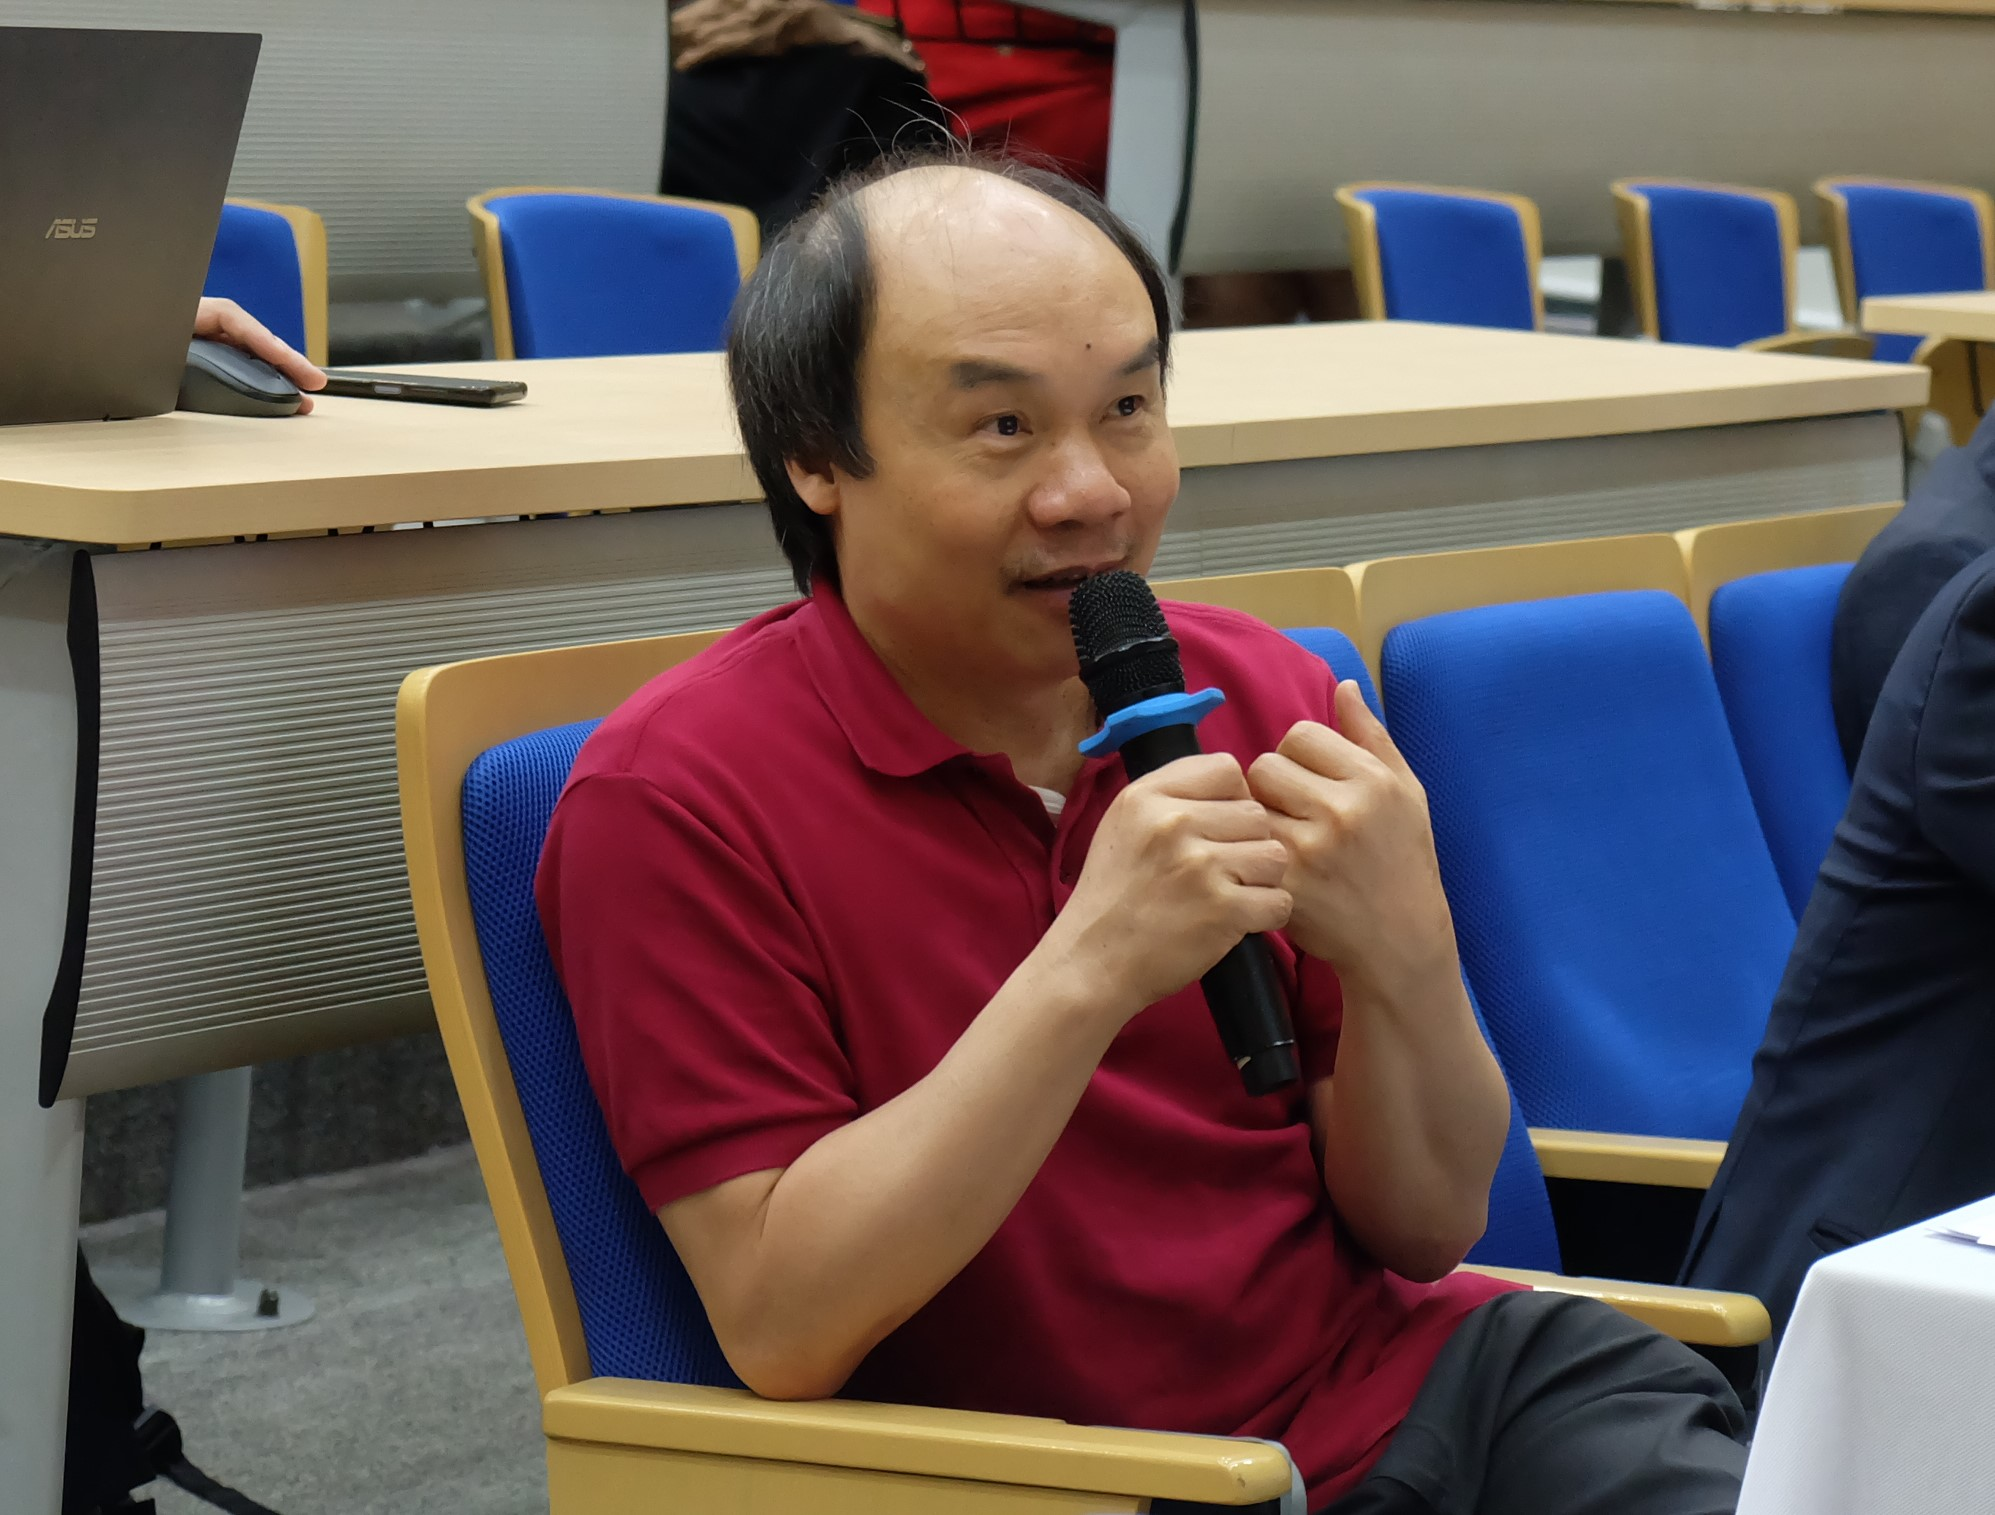
\includegraphics[width= 1\linewidth]{1.1}
		\caption{\small\textit{\color{diendantoanhoc}GS. Đỗ Đức Thái, Đại học Sư phạm Hà Nội.}}
		\vspace*{-10pt}
	\end{figure}
	Tuy nhiên, cũng từ bài giảng này, GS Thái đã cảnh báo về nguy cơ dạy học xa rời cái cốt lõi, dạy toán, mà nhiều giáo viên có thể mắc phải vì say sưa với cái gọi là ``tích hợp". Cái mà những người biên soạn Chương trình phổ thông $2018$ môn toán quan tâm là thầy cô giáo dạy toán cho học sinh, chứ không phải ra sức tô vẽ cho các bài dạy để bài học trông cho có vẻ hấp dẫn, nhưng lại không đọng lại được trong trí não người học kiến thức toán. ``Dạy toán, việc đầu tiên là dạy toán! Dạy cho tử tế toán! Rồi muốn làm việc gì thì làm sau. Học sinh học môn toán thì trước hết các em phải được học toán", GS Thái khẳng định. 
	\vskip 0.1cm
	\textbf{\color{diendantoanhoc}Phải tuân thủ những chuẩn mực} 
	\vskip 0.1cm
	Với phần trình bày của tác giả Nguyễn Thụy Việt Anh (Trường Liên cấp Hội nhập Quốc tế Ischool, Quảng Trị), về \textit{Hình có trục đối xứng}, GS Đỗ Đức Thái cảnh báo, người giáo viên luôn cần xác định một bài học cụ thể thuộc dạng nào trong lý thuyết dạy học. Trong trường sư phạm, giáo sinh được dạy cách xác định dạng bài điển hình trong lý thuyết dạy học. Bởi mỗi dạng bài điển hình sẽ có một nguyên tắc dạy học mà người dạy phải bám theo nguyên tắc đó, giống như đi đường thì phải đi bên phải.  
	\vskip 0.1cm
	``Dạy toán có những chuẩn mực về mặt sự phạm. Đây là bài học về dạy khái niệm mới, định nghĩa mới. Ở bài này, GV dạy một khái niệm rất khó với học sinh, đó là hình có trục đối xứng, hay nói cách khác, đối xứng trục mà lại không được phép định nghĩa phép đối xứng trục (vì lên đến lớp $10$ học sinh mới được học kiến thức này ở chuyên đề). Nguyên tắc dạy bài học khái niệm mới, định nghĩa mới, bao gồm nhiều bước, trong đó bước cuối cùng là làm nổi bật lên được là chốt lại, neo lại trong đầu học sinh khái niệm mới đó là cái gì", GS Thái phát biểu. 
	\vskip 0.1cm
	\textbf{\color{diendantoanhoc}Học toán để làm gì?} 
	\vskip 0.1cm
	Ngay từ bài giảng đạt giải cao nhất (giải nhì, không có giải nhất) trong phần \textit{Tìm hiểu về môn Toán trong ``Chương trình giáo dục phổ thông mới" thông qua một chủ đề cụ thể}, các thí sinh và người theo dõi cuộc thi cũng được nhận những chia sẻ thấu đáo về quan điểm dạy toán của những người tham gia biên soạn chương trình môn toán. Đây là bài giảng \textit{Giải bài toán tập hợp bằng phương pháp ``ô ăn quan"}, của nhóm tác giả Ngô Quốc Trung, Nguyễn Thị Hiền (Trường Liên cấp Hermann Gmeiner Vinh, Nghệ An). Phần đầu bài giảng, các tác giả dùng phương pháp ô ăn quan để giải các bài toán ở tiểu học (thường được gọi là bài toán giả thiết tạm). ``Tôi thấy phần đó rất thú vị, rất sáng tạo. Nó cho học sinh thấy một cơ chế mà thoát ra khỏi bản chất giải phương trình. Tôi hoàn toàn cho điểm $10$ ở phần đó", GS Thái nhận xét.
	\vskip 0.1cm
	Nhưng với phần thứ hai, các tác giả dùng phương pháp này với nội dung tổ hợp ở lớp $10$, thì các tác giả không thuyết phục được ban giám khảo. ``Nói cho cùng, học toán là học cách nghĩ, cách suy luận, cách khám phá ra một cái gì đó. Từ nó dẫn người ta đến tư duy, đến những thuật toán chung, để khái quát nó lên, giải quyết những mô hình trong cuộc sống mà nó tương tự như thế. Việc dùng một phương pháp thiên về mô tả cho nội dung tổ hợp ở lớp 10 của các tác giả vừa khiến cho bài giảng cầu kỳ, vừa không phù hợp.  Học sinh lớp $10$, $15-16$ tuổi rồi, không phải lúc nào cũng cầm nắm sờ mó với mô tả được. Một lúc nào đó, anh phải chuyển từ \textit{cụ thể} lên đến \textit{hình ảnh}, rồi lên đến \textit{biểu tượng hoá} chứ.",  GS Thái chia sẻ.
	\vskip 0.1cm
	\PIbox{Cuối tháng Ba vừa qua, trong trong khuôn khổ sự kiện "Toán học cho mọi người",  vòng chung khảo kỳ thi Bài giảng và bài viết về Toán học, mang tên Hoàng Tụy, lần thứ hai, đã được diễn ra. Trước đó, hội đồng giám khảo đã tiến hành chấm các hồ sơ dự thi ở vòng sơ khảo, lựa chọn được $8$ hồ sơ tốt nhất để tranh tài tại vòng chung khảo. Tại vòng chung khảo (diễn ra ở hội trường Hoàng Tụy, Viện Toán học Việt Nam), đại diện nhóm tác giả hoặc các tác giả đã \linebreak thuyết trình các bài giảng và bài viết trước}
	
	\PIbox{hội đồng giám khảo, trước sự theo dõi (trực tiếp và trực tuyến) của những người quan tâm tới kỳ thi. Theo hội đồng giám khảo, chất lượng hồ sơ dự thi năm nay cao hơn hẳn năm trước, vì thế mà phần trình bày của $8$ thí sinh được lựa chọn thuyết trình trong vòng chung khảo ít nhiều đều tạo sự thú vị cho người theo dõi. 
	\vskip 0.1cm	
	Trọng tâm nội dung của kỳ thi lần thứ hai là Tìm hiểu về môn Toán trong ``Chương trình giáo dục phổ thông mới" thông qua một chủ đề cụ thể. Bên cạnh đó là một số nội dung truyền thống như: Tìm hiểu về Toán sơ cấp, lịch sử Toán học và Toán học trong cuộc sống. 
	\vskip 0.1cm	
	Hội đồng giám khảo năm nay gồm GS Ngô Việt Trung, Chủ tịch Hội Toán học Việt Nam, nguyên Viện trưởng Viện Toán học; GS Đỗ Đức Thái, Trường ĐH Sư phạm Hà Nội; GS Phùng Hồ Hải, Phó chủ tịch Hội Toán học Việt Nam, nguyên Viện trưởng Viện Toán học; GS Hà Huy Khoái, nguyên Viện trưởng Viện Toán học; TS Trần Nam Dũng, Phó hiệu trưởng Trường Phổ thông Năng khiếu, ĐH Quốc gia TP.HCM; PGS Phó Đức Tài, Trưởng Khoa Toán-Cơ-Tin học, Trường ĐH Khoa học Tự nhiên, ĐH Quốc gia Hà Nội. }
	\vskip 0.1cm
	\textbf{\color{diendantoanhoc}Kết quả chung cuộc như sau:}
	\vskip 0.1cm
	\textit{Nội dung ``Tìm hiểu về môn Toán trong ``Chương trình giáo dục phổ thông mới" thông qua một chủ đề cụ thể": }
	\vskip 0.1cm
	$\bullet$	Giải nhì (không có giải nhất): Bài giảng ``Giải bài toán tập hợp bằng phương pháp ``ô ăn quan" của nhóm tác giả Ngô Quốc Trung, Nguyễn Thị Hiền, Trường Liên cấp Hermann Gmeiner Vinh, Nghệ An. 
	\vskip 0.1cm
	$\bullet$	Giải ba: Bài viết ``Một cách thiết kế dạy học Toán theo hướng gắn liền với thực tiễn", tác giả Phạm Đức Quang, Trường ĐH Sư phạm Hà Nội $2$.
	\vskip 0.1cm 
	$\bullet$	Giải khuyến khích: Bài giảng ``Hình có trục đối xứng", tác giả Nguyễn Thụy Việt Anh, Trường Liên cấp Hội nhập Quốc tế Ischool, Quảng Trị; Bài giảng ``Tích hợp tư duy công dân số trong bài giảng môn Toán", tác giả Nguyễn Thế Minh, Trường Trung học Vinschool Imperia, Hải Phòng.
	\vskip 0.1cm
	\textit{Các nội dung khác:}
	\vskip 0.1cm 
	$\bullet$	Giải nhất: Bài giảng ``Bổ đề hai đoạn thẳng và một số ứng dụng", tác giả Nguyễn Hữu Tâm, Trường THPT chuyên Lê Quý Đôn, Bình Định. 
	\vskip 0.1cm
	$\bullet$	Giải nhì: Bài giảng ``Mập mờ công thức Euler", tác giả Nguyễn Quang Minh, Biên Hoà, Đồng Nai. 
	\vskip 0.1cm
	$\bullet$	Giải ba: Bài giảng ``Lý thuyết đồ thị và một số cấu trúc đáng chú ý", tác giả Hà Trung, Trường THPT chuyên Lê Hồng Phong, Nam Định. 
	\vskip 0.1cm
	$\bullet$	Giải khuyến khích: Bài giảng ``Nét đẹp của phương pháp đếm dưới góc nhìn của số Fibonacci", tác giả Nguyễn Tuấn Anh, Trường PTTH chuyên Nguyễn Quang Diêu, Đồng Tháp. 
\end{multicols}